\documentclass[11pt,a4paper]{article}
\usepackage[margin=2.5cm]{geometry}
\usepackage[T1]{fontenc}
\usepackage{mathptmx}
\usepackage[scaled=0.9]{helvet}
\usepackage{microtype}
\usepackage{graphicx}
\usepackage{booktabs}
\usepackage{array}
\usepackage{amsmath,amssymb}
\usepackage{xcolor}
\usepackage{float}
\usepackage{caption}
\usepackage{enumitem}
\usepackage{fancyhdr}
\usepackage[numbers,sort&compress]{natbib}
\usepackage[colorlinks=true,linkcolor=blue!50!black,citecolor=blue!50!black,urlcolor=blue!50!black]{hyperref}
\usepackage{url}
\captionsetup{font=small,labelfont=bf}
\setlist{itemsep=2pt,topsep=4pt}
\graphicspath{{../results/figures/}}
\setlength{\parskip}{4pt}
\renewcommand{\arraystretch}{1.12}

\pagestyle{fancy}
\fancyhf{}
\lhead{\small ML-Based Cloud Resource Manager}
\rhead{\small Piyush Chaudhary (16010123234)}
\cfoot{\thepage}
\renewcommand{\headrulewidth}{0.4pt}

\sloppy
\begin{document}

%================ TITLE PAGE ================
\begin{titlepage}
\centering
\vspace*{1.5cm}
{\large K.J. Somaiya College of Engineering\\[2pt] Department of Computer Engineering}\\[1.2cm]
{\large Advanced Cloud Computing (ACC) --- Continuous Assessment}\\[1.5cm]
\rule{\linewidth}{1.2pt}\\[0.5cm]
{\LARGE\bfseries ML-Based Memory Usage Prediction and\\[4pt] Intelligent Cloud Resource Allocation}\\[0.5cm]
\rule{\linewidth}{1.2pt}\\[1.5cm]
{\large Design, simulation and evaluation of a forecast-driven auto-scaling resource manager}\\[2.5cm]
\begin{tabular}{rl}
\textbf{Name:} & Piyush Chaudhary\\
\textbf{Roll No.:} & 16010123234\\
\textbf{Programme:} & B.Tech Computer Engineering\\
\textbf{Source code:} & \url{https://github.com/Piyushchy/acc-lab-ca}\\
\end{tabular}\\[2cm]
{\large October 2026}
\vfill
\end{titlepage}

%================ ABSTRACT ================
\begin{abstract}
Cloud services are commonly provisioned either for their peak load, which wastes money and energy, or reactively, which adds capacity only after demand has risen and therefore risks running out of memory while new instances boot. This report designs, implements and evaluates an ML-based resource manager that forecasts the memory demand of a service 15 minutes ahead and sizes a pool of virtual machines accordingly. A leakage-free set of 32 features is built from memory, request-rate and CPU history plus calendar information. Seven forecasters are compared on a chronological hold-out; an MLP reaches a mean absolute error of 252.6~MB (1.01\,\% MAPE), about half the error of the ``no change'' baseline. The forecast, in the form of a 95th-percentile upper bound, drives a discrete-time auto-scaling simulator that is compared with static peak provisioning, reactive target tracking and an oracle on prediction accuracy, utilisation, latency, cost and energy. Dynamic scaling raises average utilisation from 50\,\% to about 78\,\% and reduces simulated cost by about 36\,\% and energy by about 21\,\%. The report then studies what happens when the prediction is wrong: systematic under-prediction is dangerous (28.9\,\% of time steps with exhausted memory at $-20\,\%$ bias), over-prediction merely costs money, and for sudden unforeseen surges the instance launch delay, not the forecaster, is the binding constraint. A drift-detecting hybrid policy removes the bias failure at a cost premium. All results use a synthetic workload and an assumed cost/power model; this limitation is stated prominently and discussed throughout.
\end{abstract}

\setcounter{tocdepth}{1}
\tableofcontents
\newpage

%================ 1 INTRO ================
\section{Introduction and Problem Statement}
Elasticity is a defining property of cloud computing: resources can be acquired and released on demand~\cite{armbrust2010}. Exploiting it requires deciding \emph{how many} resources to hold at each moment. Peak-sized (static) provisioning guarantees capacity but leaves most of it idle; reactive auto-scalers, such as the target-tracking policies of commercial platforms~\cite{awsasg}, respond to \emph{current} utilisation, so capacity arrives one launch-and-warm-up delay after the demand it was meant for~\cite{lorido2014}. Predictive approaches address this by forecasting the workload and acquiring capacity in advance~\cite{roy2011,calheiros2015,cortez2017}.

\paragraph{Problem.} Design an ML-based cloud resource manager that predicts workload and allocates resources. The assignment asks us to
\begin{enumerate}[label=(\roman*)]
  \item identify the input data and features,
  \item choose the ML algorithm and prediction horizon,
  \item design the resource-allocation / auto-scaling mechanism,
  \item evaluate prediction accuracy, utilisation, latency, cost and energy, and
  \item discuss what happens when the prediction is wrong.
\end{enumerate}
Sections~\ref{sec:data}--\ref{sec:wrong} address these items in order; Section~\ref{sec:cloud} describes the cloud demonstration.

\paragraph{Scope and honesty statement.} The default workload is \emph{synthetic} and the cluster is a \emph{discrete-time simulator} with assumed price and power figures. No headline number was measured on a live cloud account. The code can ingest any real trace and includes scripts to collect metrics on a cloud VM and to push recommendations to an AWS Auto Scaling Group, but the latter has only been run in dry-run mode. Consequently, absolute values (dollars, kWh, milliseconds) illustrate \emph{relative} differences between policies and should not be read as predictions for a real deployment.

%================ 2 DATA ================
\section{Input Data and Features}\label{sec:data}
\subsection{Workload data}
The trace covers 60 days at 5-minute resolution (17{,}280 rows) with three columns: request rate (req/s), CPU utilisation (\%) and aggregate service memory demand (MB, range 13--40~GB). The generator (\texttt{src/data\_gen.py}) combines diurnal and weekly seasonality, 12\,\% long-term growth, AR(1) noise and about one traffic burst per day; CPU is proportional to the request rate; memory is a baseline plus an exponentially smoothed response to the request rate plus a slow leak that resets at simulated deployments. Figure~\ref{fig:workload} shows the series.

The data are split \emph{chronologically}: 60\,\% train ($\approx$35 days), 20\,\% validation and 20\,\% test ($\approx$11.8 days), without shuffling, so every model is evaluated on the future relative to its training data~\cite{hyndman2018}.

\begin{figure}[H]
\centering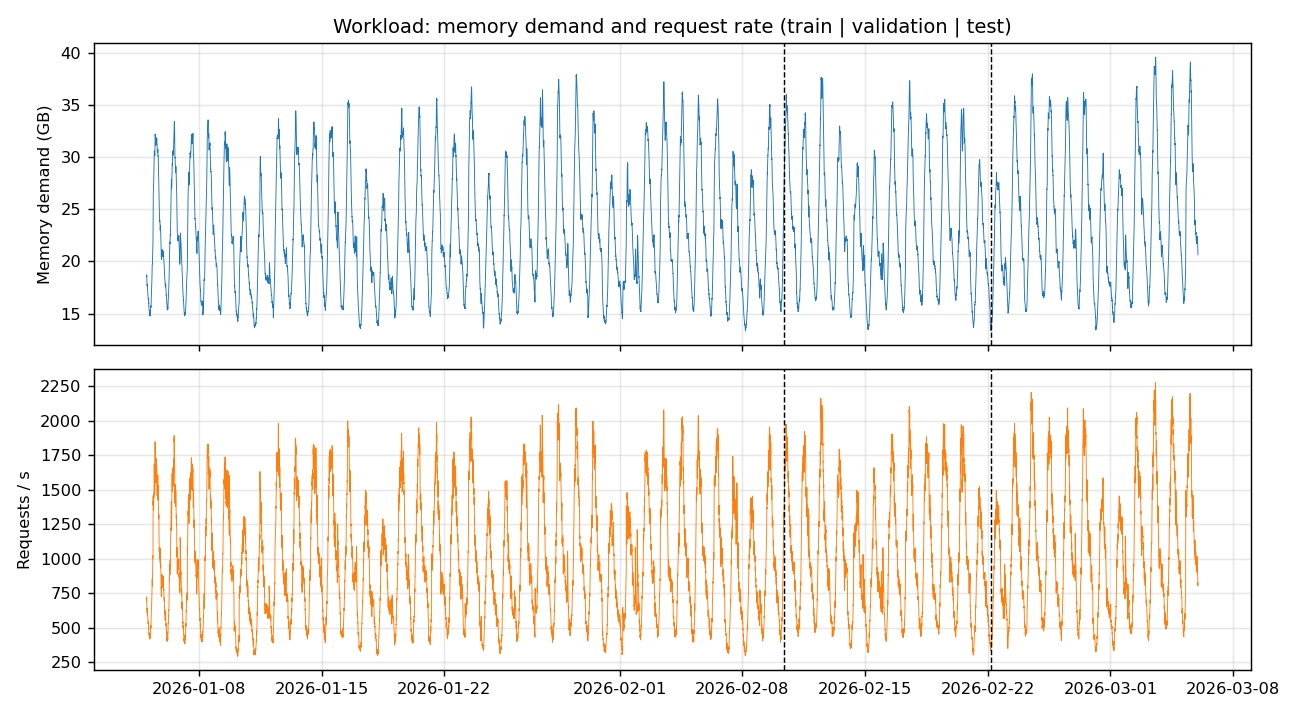
\includegraphics[width=0.92\linewidth]{01_workload.png}
\caption{Synthetic workload: request rate, CPU and memory demand, with the train/validation/test split.}\label{fig:workload}
\end{figure}

\subsection{Features}
All 32 features at time $t$ use only data available up to $t$; a unit test (\texttt{tests/test\_pipeline.py}) verifies the absence of look-ahead leakage.
\begin{itemize}
  \item \textbf{Memory history:} current level and differences over 5~min to 24~h (lags of 1, 2, 3, 6, 12, 36, 72, 144 and 288 steps).
  \item \textbf{Rolling statistics:} deviation from the mean, standard deviation and deviation from the maximum over 30~min, 1~h and 3~h windows.
  \item \textbf{Seasonal signal:} the memory change over the same window \emph{yesterday}.
  \item \textbf{Request and CPU signals:} request level, differences, exponential moving average, 3~h mean, CPU level and 15-min CPU change. Request rate is a leading indicator of memory.
  \item \textbf{Calendar features} of the \emph{target} time: $\sin/\cos$ of hour of day and day of week, and a weekend flag.
\end{itemize}

\subsection{Target}
The target is the memory \emph{change} over the horizon $h$, $y_t = m_{t+h}-m_t$; the forecast is $\hat m_{t+h}=m_t+\hat y_t$. Predicting the change rather than the level prevents tree-based models from having to extrapolate beyond the memory range seen in training, which matters because the growth trend pushes the test period above the training range.

%================ 3 ALGORITHM ================
\section{Algorithm Selection and Prediction Horizon}\label{sec:algo}
\subsection{Candidate models}
Three baselines (persistence, 1-hour moving average, seasonal-naive using yesterday's change) and four learned regressors were compared: Ridge regression~\cite{hoerl1970}, Random Forest~\cite{breiman2001}, gradient boosting (scikit-learn's histogram implementation)~\cite{friedman2001} and a two-hidden-layer MLP (64--32 units)~\cite{rumelhart1986}, all implemented with scikit-learn~\cite{pedregosa2011}. Models are fit on the training set, the best learned model is selected by \emph{validation} MAE, all models are then refit on train+validation, and the test set is scored once.

\begin{table}[H]
\centering\caption{Forecast accuracy on the held-out test period (15-minute horizon).}\label{tab:models}
\begin{tabular}{lrrrr}
\toprule
Model & MAE (MB) & RMSE (MB) & MAPE & Skill vs.\ persistence\\
\midrule
Persistence & 497.0 & 648.1 & 2.01\,\% & 0\,\%\\
Moving average (1 h) & 1249.5 & 1575.6 & 5.05\,\% & $-151$\,\%\\
Seasonal naive (24 h) & 436.8 & 597.5 & 1.75\,\% & 12.0\,\%\\
Ridge regression & 256.0 & 367.4 & 1.02\,\% & 48.5\,\%\\
Random Forest & 259.5 & 372.0 & 1.03\,\% & 47.8\,\%\\
Gradient Boosting & 260.5 & 371.8 & 1.03\,\% & 47.6\,\%\\
\textbf{MLP (64--32)} & \textbf{252.6} & \textbf{361.9} & \textbf{1.01\,\%} & \textbf{49.2\,\%}\\
\bottomrule
\end{tabular}
\end{table}

The four learned models lie within about 3\,\% of each other and a linear model is competitive. This is expected because the synthetic memory is generated by nearly linear dynamics; Table~\ref{tab:models} therefore says little about which model family would win on real traces. The MLP was selected by the validation rule. Figures~\ref{fig:modelcmp} and~\ref{fig:fva} show the comparison and the forecast against the actual series.

\begin{figure}[H]
\centering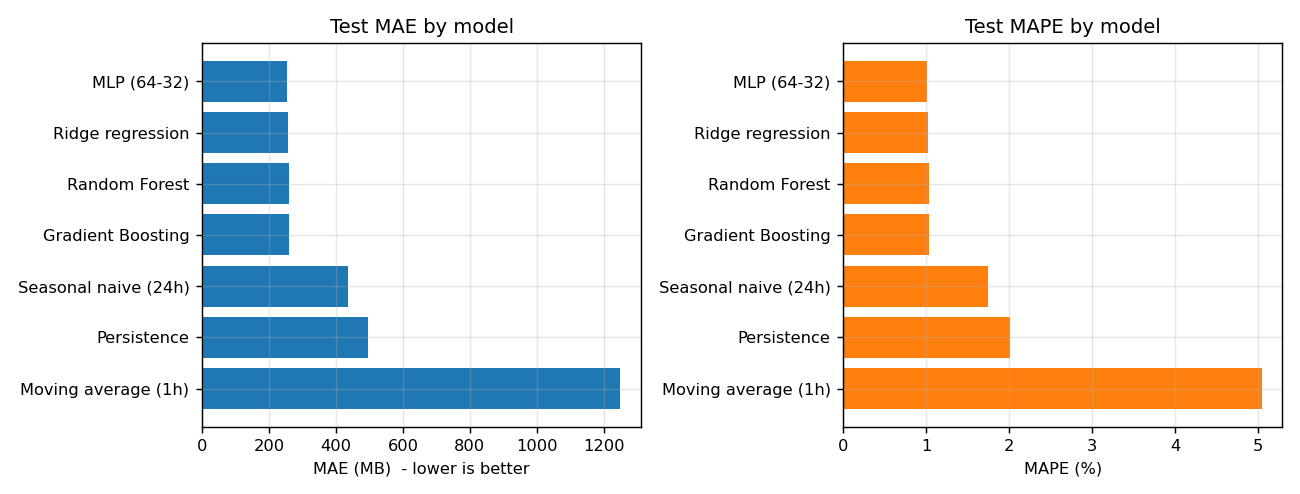
\includegraphics[width=0.9\linewidth]{02_model_comparison.png}
\caption{Model comparison on the test set.}\label{fig:modelcmp}
\end{figure}
\begin{figure}[H]
\centering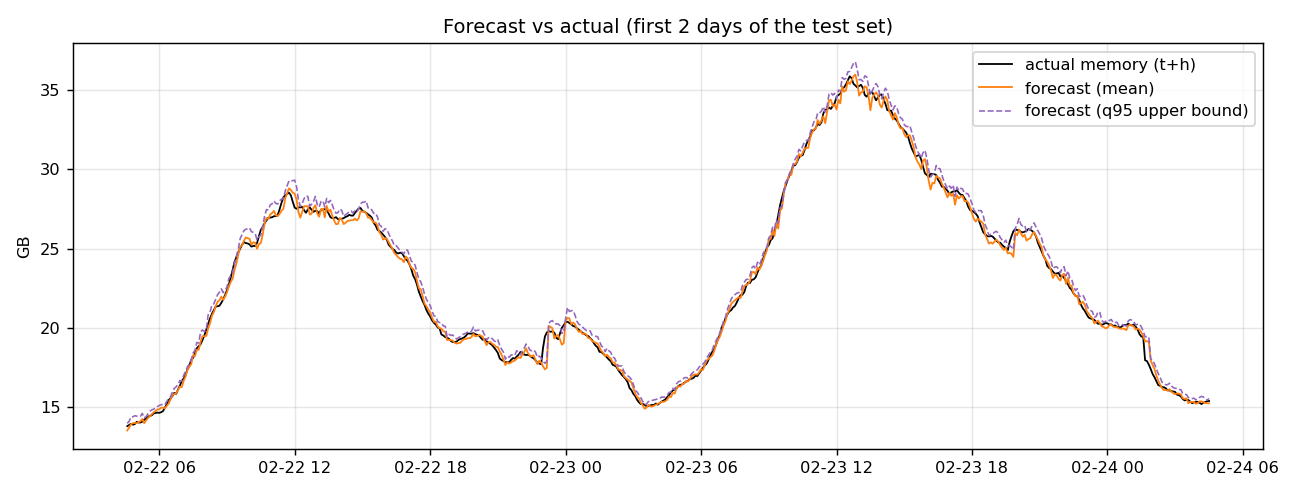
\includegraphics[width=0.9\linewidth]{03_forecast_vs_actual.png}
\caption{Forecast versus actual memory over part of the test period.}\label{fig:fva}
\end{figure}

\subsection{Upper-bound model}
Capacity must cover the demand that actually occurs, not its mean, so a gradient-boosting \emph{quantile} model ($q=0.95$)~\cite{koenker1978} supplies an upper bound. On the test set its empirical coverage is 90.8\,\% rather than the nominal 95\,\%: it is somewhat over-confident, plausibly because of the upward trend between training and test periods. A conformal calibration step would be a natural improvement. Permutation importance (Figure~\ref{fig:imp}) ranks the target-time hour, short-term request-rate changes and the weekend flag highest.

\begin{figure}[H]
\centering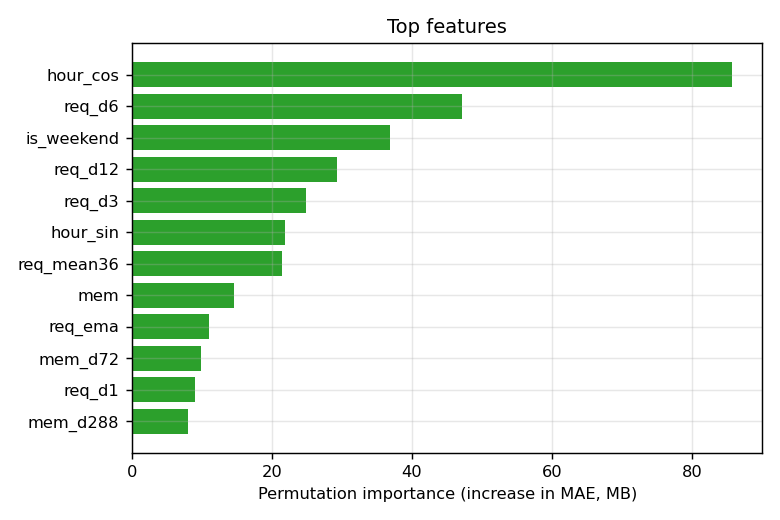
\includegraphics[width=0.62\linewidth]{04_feature_importance.png}
\caption{Permutation feature importance.}\label{fig:imp}
\end{figure}

\subsection{Prediction horizon}
The default horizon is \textbf{15 minutes (3 steps)}, equal to the assumed instance launch and warm-up time: a decision made now only matters for the moment the new capacity becomes available. Table~\ref{tab:horizon} and Figure~\ref{fig:horizon} sweep the horizon.

\begin{table}[H]
\centering\caption{Effect of the prediction horizon (hybrid policy).}\label{tab:horizon}
\begin{tabular}{lrrrrr}
\toprule
Horizon & 5 min & 10 min & 15 min & 30 min & 60 min\\
\midrule
Forecast MAE (MB) & 97 & 176 & 261 & 489 & 810\\
Persistence MAE (MB) & 179 & 340 & 497 & 942 & 1756\\
Cost (USD) & 91.7 & 92.2 & 92.7 & 93.5 & 94.7\\
Steps with memory exhausted & 0\,\% & 0\,\% & 0\,\% & 0\,\% & 0\,\%\\
\bottomrule
\end{tabular}
\end{table}
Error grows roughly linearly with the horizon and cost rises slightly because more headroom is needed. On this smooth series, horizons shorter than the launch delay did not cause violations, so the 15-minute choice rests on the launch-delay argument rather than on a measured penalty.

\begin{figure}[H]
\centering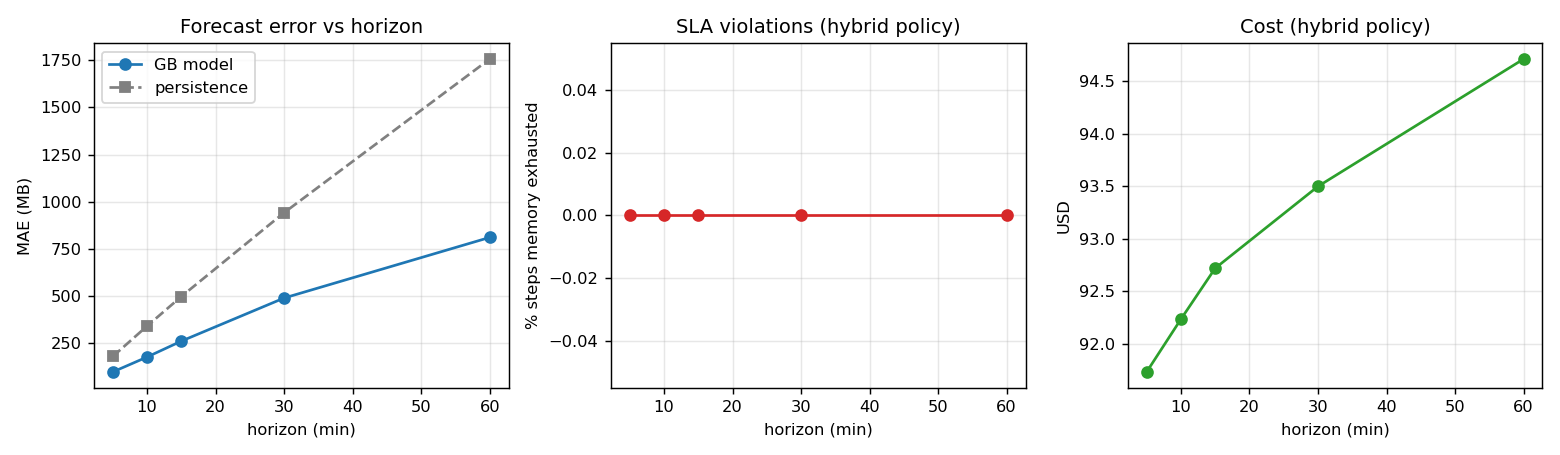
\includegraphics[width=0.95\linewidth]{09_horizon_sweep.png}
\caption{Horizon sweep: forecast error and policy cost.}\label{fig:horizon}
\end{figure}

%================ 4 DESIGN ================
\section{Resource Allocation and Auto-Scaling Mechanism}\label{sec:design}
The simulated service runs on instances of 4~GB memory with a 15-minute launch and warm-up delay and a pool of 2--80 instances. At each 5-minute step the controller applies:
\begin{enumerate}
  \item \textbf{Sizing rule.}
  \begin{equation}
    N_t=\left\lceil \frac{\hat m^{(0.95)}_{t+h}}{M_{\text{inst}}\cdot u^\star}\right\rceil,\qquad M_{\text{inst}}=4096\,\text{MB},\;u^\star=0.85,
  \end{equation}
  where $\hat m^{(0.95)}_{t+h}$ is the q95 forecast (the mean forecast is used for the ``predictive-mean'' policy).
  \item \textbf{Immediate scale-out.} The request is issued at once, but capacity arrives only after the launch delay; billing and idle power start at launch.
  \item \textbf{Stabilised scale-in.} The pool shrinks only to the highest desired size seen in the last 30 minutes (anti-flapping), identically for all dynamic policies.
  \item \textbf{Safety nets (hybrid policy).} An emergency guard acts on current utilisation, and a drift fallback replaces the model when realised error is high (Section~\ref{sec:wrong}).
\end{enumerate}

\paragraph{Policies compared.} (1) \emph{Static}: training peak plus 20\,\%, i.e.\ 12 instances; (2) \emph{Reactive}: the same sizing rule fed with \emph{current} demand (target tracking); (3) \emph{Predictive (mean)}; (4) \emph{Predictive (q95)}; (5) \emph{Hybrid}: q95 plus safety nets; (6) \emph{Oracle}, which knows the true demand at $t+h$ and bounds what any forecaster can achieve.

%================ 5 METRICS ================
\section{Evaluation Methodology}\label{sec:metrics}
\begin{itemize}
  \item \textbf{Prediction accuracy:} MAE, RMSE, MAPE, $R^2$, skill versus persistence, under-prediction rate and q95 coverage.
  \item \textbf{Utilisation:} mean of $\min(\text{demand}/\text{capacity},1)$.
  \item \textbf{Reliability:} percentage of steps in which demand exceeds capacity (memory exhausted), number of such episodes and shortfall in GB-hours.
  \item \textbf{Latency (proxy):} $40\,\text{ms}/(1-u)$, capped at 20$\times$ below saturation and set to 2000~ms when memory is exhausted; mean, p95 and p99 are reported.
  \item \textbf{Cost:} billed instance-hours at \$0.0416 per instance-hour.
  \item \textbf{Energy:} per-instance power rising linearly from 45~W idle to 110~W at full utilisation~\cite{barroso2007}; booting instances draw idle power.
\end{itemize}
Prices, power numbers and the latency model are \emph{assumptions}. The latency proxy is a queueing-style heuristic, not a measurement.

%================ 6 RESULTS ================
\section{Results}\label{sec:results}
\begin{table}[H]
\centering\caption{Policy comparison on the test period (85\,\% sizing target).}\label{tab:policies}
\small
\begin{tabular}{lrrrrrr}
\toprule
Policy & Util. & Mem.\ exhausted & p99 (ms) & Cost (\$) & Energy (kWh) & Avg inst.\\
\midrule
Static (peak-sized) & 50.3\,\% & 0\,\% & 194 & 141.36 & 264.0 & 12.0\\
Reactive & 78.6\,\% & 0.03\,\% & 333 & 90.95 & 209.5 & 7.7\\
Predictive (mean) & 78.5\,\% & 0\,\% & 279 & 90.95 & 209.5 & 7.7\\
Predictive (q95) & 77.0\,\% & 0\,\% & 255 & 92.71 & 211.4 & 7.8\\
Hybrid & 77.0\,\% & 0\,\% & 254 & 92.72 & 211.4 & 7.8\\
Oracle & 78.5\,\% & 0\,\% & 263 & 90.98 & 209.5 & 7.7\\
\bottomrule
\end{tabular}
\end{table}

\begin{figure}[H]
\centering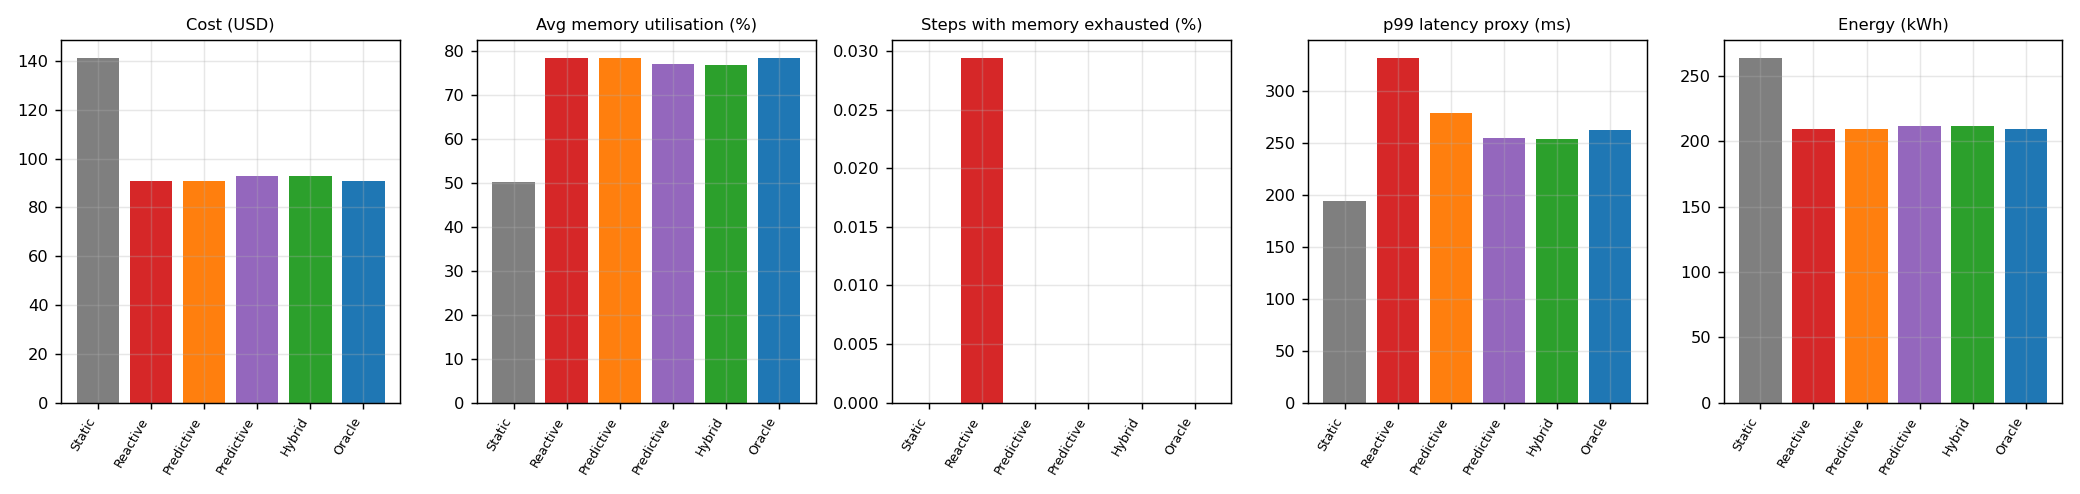
\includegraphics[width=\linewidth]{05_policy_comparison.png}
\caption{Utilisation, violations, latency, cost and energy by policy.}\label{fig:policy}
\end{figure}

Every dynamic policy reduces cost by about 36\,\% and energy by about 21\,\% relative to static peak sizing, at the price of higher latency because the cluster runs hotter, which the latency proxy penalises. At the default 85\,\% target the differences between reactive and ML policies are small: slow diurnal ramps fit within 15\,\% headroom even with a 15-minute delay. The ML policies avoid the single short reactive violation and lower p99 latency, at equal cost for the mean forecast and +2\,\% for the q95 headroom. Figure~\ref{fig:timeline} shows capacity tracking demand.

\begin{figure}[H]
\centering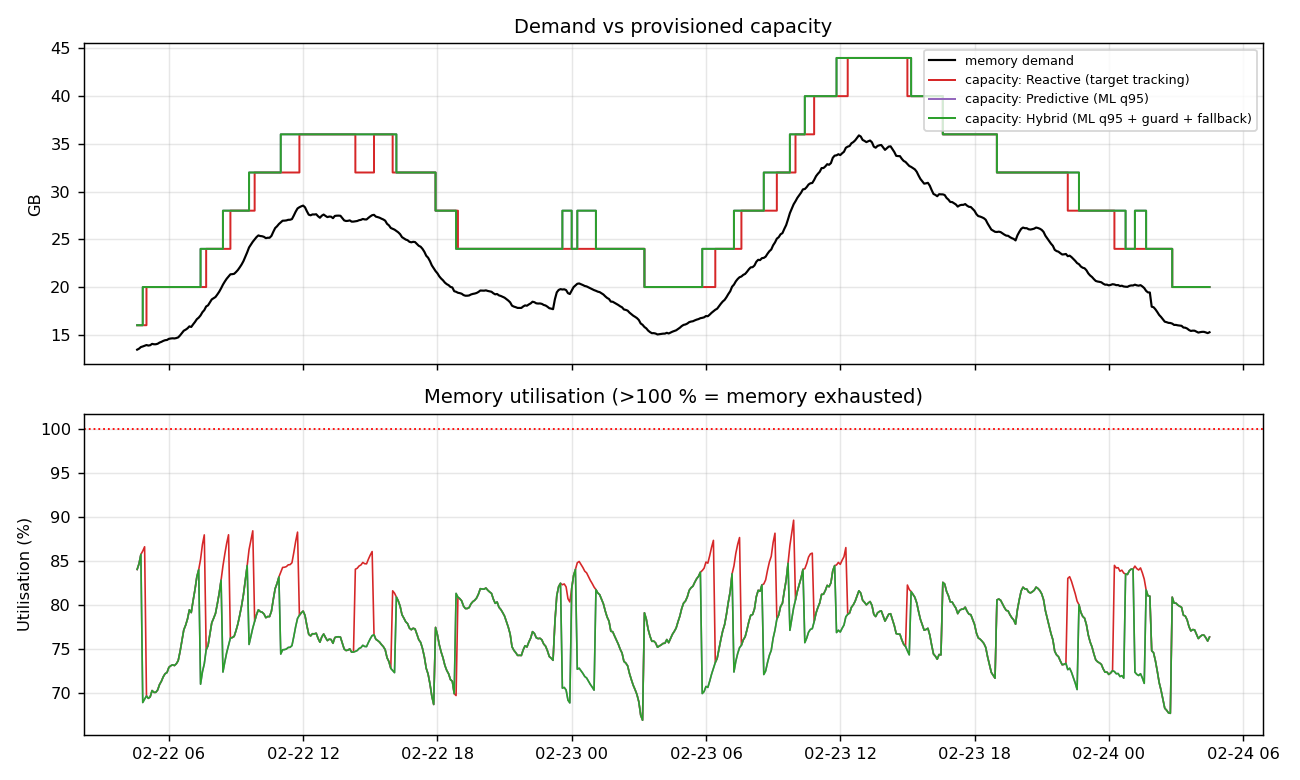
\includegraphics[width=0.9\linewidth]{06_capacity_timeline.png}
\caption{Capacity versus demand over time for the compared policies.}\label{fig:timeline}
\end{figure}

\subsection{Where prediction matters: tighter packing}
Because the default target hides differences, the sizing target $u^\star$ was swept (Table~\ref{tab:sweep}, Figure~\ref{fig:sweep}). The forecast allows tighter packing with fewer violations at nearly the same cost; the benefit is real in this simulation but small in absolute terms (fractions of a percent of steps). The sweep was added after a first run at a 75\,\% target showed zero violations for all dynamic policies; all points are reported, not only favourable ones.

\begin{table}[H]
\centering\caption{Sizing-target sweep, normal workload.}\label{tab:sweep}
\begin{tabular}{rrrrr}
\toprule
 & \multicolumn{2}{c}{Reactive} & \multicolumn{2}{c}{Predictive (mean)}\\
\cmidrule(lr){2-3}\cmidrule(lr){4-5}
Target $u^\star$ & Violations & Cost (\$) & Violations & Cost (\$)\\
\midrule
70\,\% & 0\,\% & 109.1 & 0\,\% & 109.1\\
85\,\% & 0.03\,\% & 91.0 & 0\,\% & 91.0\\
90\,\% & 0.06\,\% & 86.0 & 0\,\% & 86.1\\
95\,\% & 0.24\,\% & 82.1 & 0.03\,\% & 82.3\\
\bottomrule
\end{tabular}
\end{table}
\begin{figure}[H]
\centering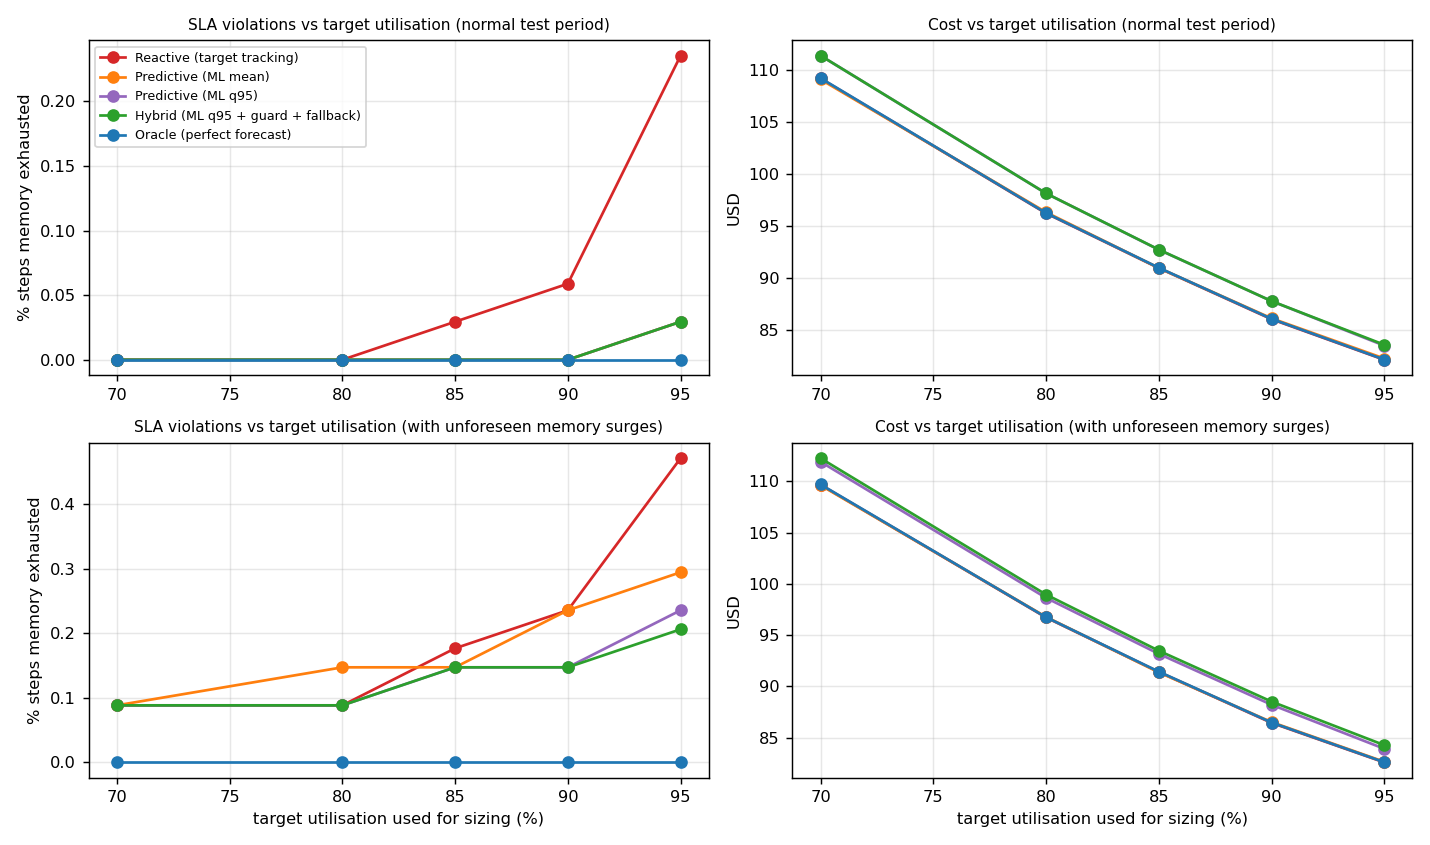
\includegraphics[width=0.85\linewidth]{10_target_util_sweep.png}
\caption{Sizing-target sweep.}\label{fig:sweep}
\end{figure}

%================ 7 WRONG ================
\section{What Happens When the Prediction Is Wrong?}\label{sec:wrong}
Four experiments probe failure behaviour (Figures~\ref{fig:wrong}, \ref{fig:shock}, \ref{fig:delay}).

\subsection{Systematic bias}
The forecast was multiplied by a constant factor (Table~\ref{tab:bias}). A 10\,\% under-forecast is still safe because of sizing headroom, but at $-20\,\%$ the predictive-only policy leaves memory exhausted in 28.9\,\% of steps (121 episodes) and at $-40\,\%$ in essentially all steps. Over-prediction is safe but costly: $+40\,\%$ raises cost from \$91 to \$125 (+37\,\%) with no violations. \textbf{Under-prediction is the dangerous direction; over-prediction only wastes money}, an asymmetry that favours an upper quantile over the mean.

\begin{table}[H]
\centering\caption{Effect of a multiplicative forecast bias (factor applied to the forecast).}\label{tab:bias}
\small
\begin{tabular}{rrrrrr}
\toprule
 & \multicolumn{2}{c}{Predictive only} & \multicolumn{2}{c}{Hybrid (drift fallback)}\\
\cmidrule(lr){2-3}\cmidrule(lr){4-5}
Factor & Mem.\ exhausted & Cost (\$) & Mem.\ exhausted & Cost (\$)\\
\midrule
0.6 & 99.97\,\% & 56.8 & 0.09\,\% & 116.4\\
0.7 & 88.08\,\% & 65.5 & 0.09\,\% & 116.4\\
0.8 & 28.87\,\% & 74.0 & 0\,\% & 116.4\\
0.9 & 0.03\,\% & 82.8 & 0\,\% & 85.9\\
1.0 & 0\,\% & 91.0 & 0\,\% & 92.7\\
1.2 & 0\,\% & 107.9 & 0\,\% & 116.4\\
1.4 & 0\,\% & 125.0 & 0\,\% & 127.2\\
\bottomrule
\end{tabular}
\end{table}

\subsection{Random noise}
Multiplicative noise of up to 20\,\% on the forecast causes no violations, but cost rises from \$91 to \$111 as the policy over-provisions on noisy up-swings; at 30\,\% noise the predictive-only policy reaches 0.18\,\% violations while the hybrid stays at 0\,\%.

\begin{figure}[H]
\centering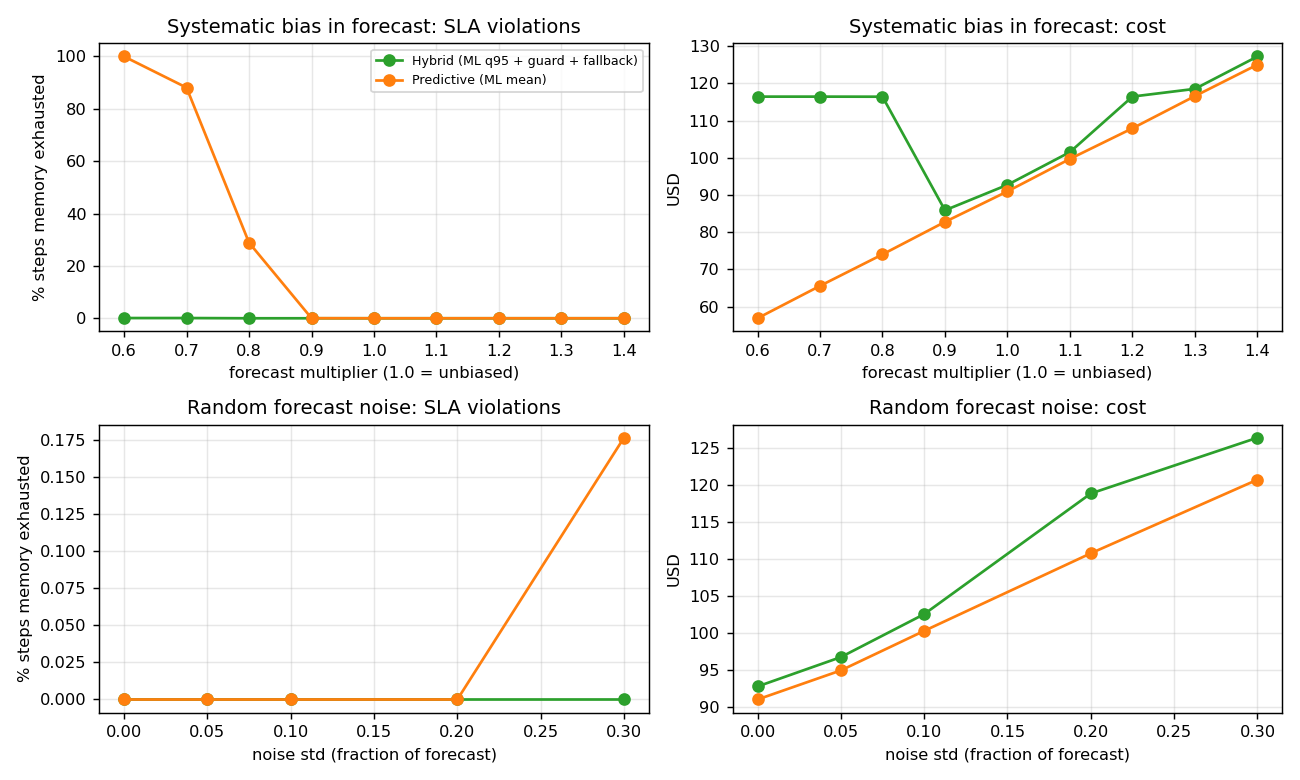
\includegraphics[width=0.9\linewidth]{07_wrong_predictions.png}
\caption{Wrong-prediction experiments: bias and noise.}\label{fig:wrong}
\end{figure}

\subsection{Unforeseen surges}
A $+40\,\%$ memory surge for 90 minutes and a $+60\,\%$ surge for 60 minutes were injected into the test period without changing the request rate, so no feature can foresee them (Table~\ref{tab:shock}, Figure~\ref{fig:shock}). Memory is exhausted in 0.18\,\% of steps for the reactive policy and 0.15\,\% for predictive and hybrid; the oracle has none. \textbf{The safety nets did not help here}: the emergency guard and the drift fallback fired (in 0.2\,\% and 0.6\,\% of steps), but new capacity still needs 15 minutes to arrive. The launch-delay sweep (Table~\ref{tab:delay}, Figure~\ref{fig:delay}) confirms that the delay is the binding constraint: with identical forecasts, violations grow from 0.03\,\% (5-minute launch) to 0.41\,\% (30 minutes), while the oracle goes from 0\,\% to 0.18\,\%.

\begin{table}[H]
\centering\caption{Surge scenario (unforeseeable memory spikes).}\label{tab:shock}
\begin{tabular}{lrrrr}
\toprule
Policy & Mem.\ exhausted & Episodes & p99 (ms) & Cost (\$)\\
\midrule
Static & 0\,\% & 0 & 195 & 141.36\\
Reactive & 0.18\,\% & 3 & 341 & 91.42\\
Predictive (mean) & 0.15\,\% & 2 & 283 & 91.38\\
Predictive (q95) & 0.15\,\% & 2 & 260 & 93.18\\
Hybrid & 0.15\,\% & 2 & 259 & 93.49\\
Oracle & 0\,\% & 0 & 263 & 91.44\\
\bottomrule
\end{tabular}
\end{table}
\begin{figure}[H]
\centering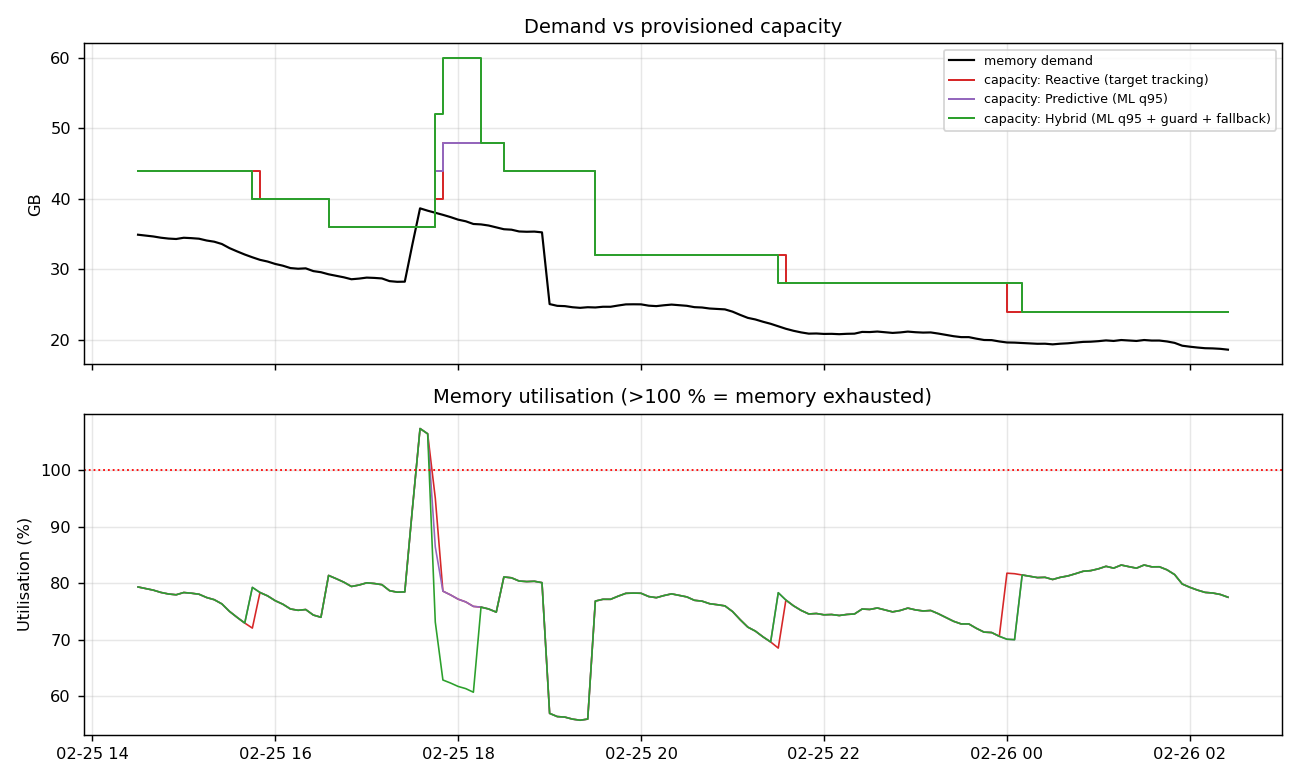
\includegraphics[width=0.85\linewidth]{08_shock_scenario.png}
\caption{Surge scenario: demand and capacity.}\label{fig:shock}
\end{figure}

\begin{table}[H]
\centering\caption{Violations (\% of steps) versus instance launch delay in the surge scenario.}\label{tab:delay}
\begin{tabular}{rrrrr}
\toprule
Launch delay (min) & Reactive & Predictive (mean) & Hybrid & Oracle\\
\midrule
5 & 0.03 & 0.03 & 0.03 & 0\\
10 & 0.09 & 0.09 & 0.09 & 0\\
15 & 0.18 & 0.15 & 0.15 & 0\\
30 & 0.44 & 0.41 & 0.41 & 0.18\\
\bottomrule
\end{tabular}
\end{table}
\begin{figure}[H]
\centering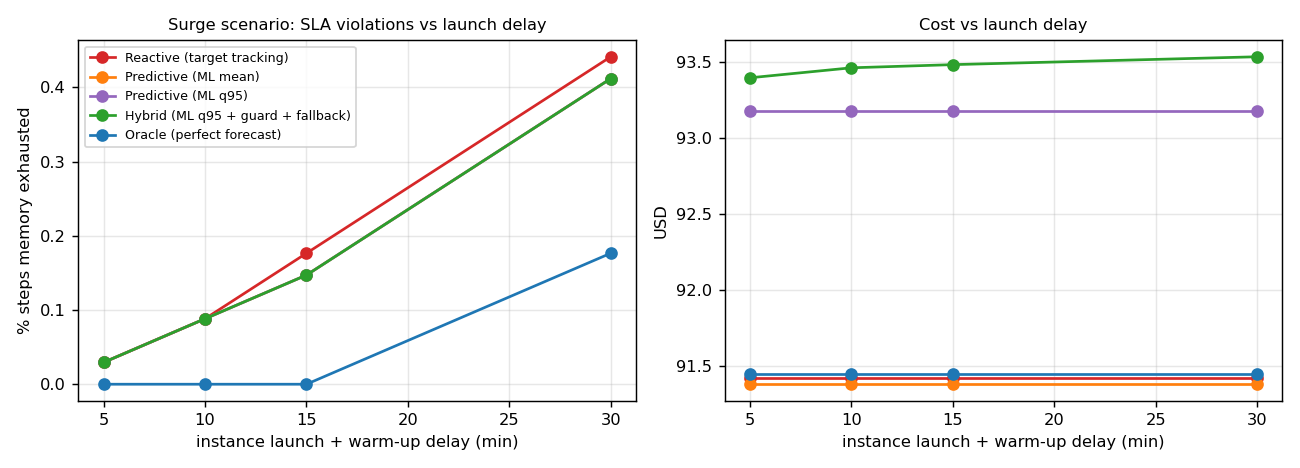
\includegraphics[width=0.9\linewidth]{11_launch_delay_sweep.png}
\caption{Launch-delay sweep in the surge scenario.}\label{fig:delay}
\end{figure}

\subsection{Drift fallback}
The hybrid compares each forecast with the value that actually occurred $h$ steps later. If the mean absolute percentage error over the last hour exceeds 12\,\%, it stops trusting the model and sizes reactively with 30\,\% headroom. With a $-20\,\%$ biased forecast the hybrid keeps violations at 0\,\% (versus 28.9\,\% for predictive-only) at \$116 versus \$93 for the unbiased hybrid: insurance paid for in cost. In the unbiased run it never triggered, so it produced no false alarms on this data.

\subsection{Mitigations}
\begin{enumerate}
  \item Forecast an upper quantile rather than the mean (implemented).
  \item Monitor realised forecast error, fall back to reactive sizing, and retrain when error stays high (fallback implemented; automated retraining is the intended operational response but is not implemented).
  \item Emergency guard on current utilisation (implemented).
  \item Minimum-capacity floor and stabilised scale-in (implemented).
  \item Shorter effective launch time through pre-warmed pools, smaller images or containers, or standing headroom. Not implemented, but indicated by the surge experiments: no policy can react faster than capacity can be created.
  \item Application-level protection such as memory limits and request shedding.
\end{enumerate}

%================ 8 CLOUD ================
\section{Cloud Demonstration}\label{sec:cloud}
The repository supports the demonstration on any cloud platform (instructions in \texttt{README.md} and \texttt{docs/DEMO\_SCRIPT.md}):
\begin{enumerate}
  \item create a small VM (AWS EC2, Google Compute Engine or Azure VM), clone the repository and install \texttt{requirements-cloud.txt};
  \item run \texttt{python main.py} to reproduce the results, or use the provided \texttt{Dockerfile};
  \item generate a real memory workload with \texttt{cloud/load\_generator.py}, record it with \texttt{cloud/collect\_metrics.py}, and retrain with \texttt{python main.py --data data/collected\_vm.csv};
  \item optionally apply the recommendation to an Auto Scaling Group with \texttt{cloud/aws\_apply.py} (dry run by default) and publish the forecast as a CloudWatch custom metric.
\end{enumerate}
\paragraph{Status.} Steps 1--3 were exercised locally, including the \texttt{--data} path; \texttt{aws\_apply.py} was run only in dry-run mode and has not been tested against a live AWS account. Seven automated tests pass (\texttt{pytest}). The screencast follows the script in \texttt{docs/DEMO\_SCRIPT.md}.

%================ 9 LIMITATIONS ================
\section{Limitations}
\begin{itemize}
  \item The data are synthetic, with a built-in ``requests lead memory'' relationship and near-linear dynamics. Real traces are less predictable, real accuracy will be lower and the model ranking may change.
  \item Costs, power and latency use assumed parameters; the simulator ignores spot pricing, billing granularity, multi-dimensional resources (CPU, network), bin-packing and application behaviour.
  \item One random seed (42) and one test window; no confidence intervals. Policy differences at the default operating point are small.
  \item The q95 model is under-covered (90.8\,\%).
\end{itemize}

%================ 10 CONCLUSION ================
\section{Conclusion}
Short-horizon memory forecasting (about 1\,\% MAPE here, roughly half the error of ``no change'') combined with an upper-quantile sizing rule lets a cluster run at about 78\,\% utilisation instead of 50\,\%, cutting simulated cost by about a third and energy by about a fifth relative to peak provisioning, with violation rates at or below those of a reactive autoscaler. The experiments also expose the limits: when forecasts are biased low, a predictive-only policy fails badly and needs the drift fallback, and when the surprise is a sudden surge, the instance launch delay rather than the forecasting method limits what any policy can achieve. Future work includes validation on real production traces, conformal calibration of the upper bound, automated retraining, multi-resource forecasting and live-cloud measurements.

\bibliographystyle{unsrtnat}
\bibliography{references}

\end{document}
